\documentclass{article}

\usepackage[margin=1in]{geometry}
\usepackage[colorlinks,linkcolor=blue,filecolor=blue,citecolor=magenta,urlcolor=blue]{hyperref}
\usepackage{bm,amsmath,amsthm,amssymb,multicol,algorithmic,algorithm,enumitem,graphicx,subfigure}
\usepackage{xargs}
\usepackage{stmaryrd}
\usepackage{natbib}

\def\M{\mathcal{M}}
\def\A{\mathcal{A}}
\def\Z{\mathcal{Z}}
\def\S{\mathcal{S}}
\def\D{\mathcal{D}}
\def\R{\mathcal{R}}
\def\P{\mathcal{P}}
\def\K{\mathcal{K}}
\def\E{\mathbb{E}}
\def\F{\mathfrak{F}}
\def\l{\boldsymbol{\ell}}

\newtheorem{Fact}{Fact}
\newtheorem{Lemma}{Lemma}
\newtheorem{Prop}{Proposition}
\newtheorem{Theorem}{Theorem} 
\newtheorem{Def}{Definition}
\newtheorem{Corollary}{Corollary}
\newtheorem{Conjecture}{Conjecture}
\newtheorem{Property}{Property}
\newtheorem{Observation}{Observation}
\newtheorem{Exa}{Example}
\newtheorem{assumption}{H\!\!}
\newtheorem{Remark}{Remark}
\newtheorem*{Lemma*}{Lemma}
\newtheorem*{Theorem*}{Theorem}
\newtheorem*{Corollary*}{Corollary}
 
\newcommand{\eqsp}{\;}
\newcommand{\beq}{\begin{equation}}
\newcommand{\eeq}{\end{equation}}
\newcommand{\eqdef}{\mathrel{\mathop:}=}
\def\EE{\mathbb{E}}
\newcommand{\norm}[1]{\left\Vert #1 \right\Vert}
\newcommand{\pscal}[2]{\left\langle#1\,|\,#2 \right\rangle}
\def\major{\mathsf{M}}
\def\rset{\ensuremath{\mathbb{R}}}




\begin{document}



\title{Layerwise and Dimensionwise Adaptive Local AMSMethod for Federated Learning}

% \author{\textbf{Belhal Karimi, Xiaoyun Li, Ping Li} \\\\
% Cognitive Computing Lab\\
% Baidu Research\\
%   10900 NE 8th St. Bellevue, WA 98004, USA
% }

\date{}
\maketitle

\begin{abstract}
To be completed...
\end{abstract}

\section{Introduction}\label{sec:introduction}

A growing and important task while learning models on observed data, is the ability to train the latter over a large number of clients which could either be devices or distinct entities.
In the paradigm of Federated Learning (FL)~\citep{konevcny2016federated,mcmahan2017communication}, the focus of our paper, a central server orchestrates the optimization over those clients under the constraint that the data can neither be centralized nor shared among the clients.
Most modern machine learning tasks can be casted as a large finite-sum optimization problem written as:
\begin{equation}
\min \limits_{\theta \in \Theta} \frac{1}{n} \sum_{i=1}^n f_i(\theta)
\end{equation}
where $n$ denotes the number of workers, $f_i$ represents the average loss for worker $i$ and $\theta$ the global model parameter taking value in $\Theta$ a subset of $\mathbb{R}^d$.
While this formulation recalls that of distributed optimization, the core principle of FL is different that standard distributed paradigm.

FL currently suffers from two bottlenecks: communication efficiency and privacy.
We focus on the former in this paper.
While local updates, updates during which each client learn their local models, can reduce drastically the number of communication rounds between the central server and devices, new techniques must be employed to tackle this challenge.
Some quantization~\citep{alistarh2017qsgd, wangni2018gradient} or compression~\citep{lin2017deep} methods allow to decrease the number of bits communicated at each round and are efficient method in a distributed setting.
The other approach one can take is to accelerate the local training on each device and thus sending a better local model to the server at each round.

Under the important setting of heterogenous data, i.e. the data among each device can be distributed according to different distributions, current local optimization algorithms are perfectible.
The most popular method for FL is using multiple local Stochastic Gradient Descent (\textsc{SGD}) steps in each device, sending those local models to the server that computes the average over those received local vector of parameters and broadcasts it back to the devices. This is called \textsc{FedAvg} and has been introduced in~\citep{mcmahan2017communication}.

In \citep{chen2020toward}, the authors motivate the usage of adaptive gradient optimization methods as a better alternative to the standard \textsc{SGD} inner loop in \textsc{FedAvg}.
They propose an adaptive gradient method, namely \textsc{Local AMSGrad}, with communication cost sublinear in $T$ that is guaranteed to converge to stationary points in $\mathcal{O}(\sqrt{d/Tn})$, where T is the number of iterations.

Based on recent progress in adaptive methods for accelerating the training procedure, see~\citep{you2019large}, we propose a variant of \textsc{Local AMSGrad} integrating dimensionwise and layerwise adaptive learning rate in each device's local update.
Our contributions are as follows:
\begin{itemize}
\item We develop a novel optimization algorithm for federated learning, namely \textsc{Fed-LAMB}, following a principled layerwise adaptation strategy to accelerate training of deep neural networks.
\item theoretical results
\item We exhibit the advantages of our method on several benchmarks supervised learning methods on both homogeneous and heterogeneous settings.
\end{itemize}

\subsection{Related Work}\label{sec:related}

\paragraph{Federated learning.}



\paragraph{Adaptive gradient methods.}


\section{Layerwise and Dimensionwise Adaptive Methods}\label{sec:main}

%\subsection{Local SGD with LARS}

\subsection{Local AMS with LAMB}

We propose a layerwise and dimensionwise local AMS algorithm in the following:

\begin{algorithm}[H]
\caption{\textsc{L\&D Local AMS for Federated Learning}} \label{alg:ldams}
\begin{algorithmic}[1]
%\small
\STATE \textbf{Input}: parameter $\beta_1$, $\beta_2$, and learning rate $\alpha_t$. 
\STATE Init: $\theta_{0} \in \Theta \subseteq \mathbb R^d $, as the global model shared by all devices and $v_{0} = \epsilon 1 \in \mathbb R^{d}$ and $\bar{\theta}_0 =  \frac{1}{n} \sum_{i=1}^n \theta_0$.
\FOR{$r=1$ to $R$}
\STATE Set $\theta_{r,i}^{0} = \bar{\theta}_{r-1}$
\STATE\textbf{parallel for device $d \in D^{r}$ do}:
\STATE Compute stochastic gradient $g_{r,i}$ at $\theta_r$.
\quad \quad \FOR{$t=1$ to $T$}
\STATE $m^t_{r,i} = \beta_1 m^{t-1}_{r-1,i} + (1 - \beta_1) g_{r,i}$.
\STATE $m^{t}_{r,i}=m^{t}_{r,i} /\left(1-\beta_{1}^{r}\right)$.
\STATE $v^{t,i}_r = \beta_2 v^{t}_{r-1,i} + (1 - \beta_2) g_{r,i}^2$.
\STATE $v^{t}_{r,i}=v^{t}_{r,i} /\left(1-\beta_{2}^{r}\right)$.
\STATE $\hat{v}^{t}_{r,i} = \max( \hat{v}^{t}_{r-1,i} , v_{r,i} )$.
\STATE Compute ratio  $p^j_{r,i}=\frac{m^{t}_{r}}{\sqrt{v^{t}_{r,i}}+\epsilon}$.
\STATE Update local model for each layer $\ell$:
$$\theta_{r,i}^{j,t}=\theta_{r,i}^{\ell,t-1}-\alpha_{r} \phi(\|\theta_{r,i}^{\ell,t-1}\|)(p_{r,i}^{j}+\lambda \theta_{r,i}^{\ell,t-1}) / \|p_{r,i}^{\ell}+\lambda \theta_{r,i}^{\ell,t-1}\|$$
\ENDFOR
\STATE Devices send local model $\theta_{r,i}^{j,T}$ to the server
\STATE Server computes the averages of the local models $\bar{\theta}_r^j = \frac{1}{n} \sum_{i=1}^n \theta_{r,i}^{j,T}$ and send it back to the devices.
\ENDFOR
\end{algorithmic}
\end{algorithm}


\subsection{Finite time convergence bounds}

In the context of nonconvex stochastic optimization for distributed devices, assume the following:

\begin{assumption}\label{ass:smooth}
For $i \in \inter$ and $\ell \in \interl$, $f_i$ is  L-smooth: $\norm{\nabla f_i (\theta) - \nabla f_i (\vartheta)} \leq L_\ell \norm{\theta^\ell-\vartheta^\ell}$.
\end{assumption}
We add some classical assumption in the unbiased stochastic optimization realm, on the gradient of the objective function:
\begin{assumption}
The stochastic gradient is unbiased for any iteration $r>0$: $\EE[g_r] = \nabla f(\theta_r)$ and is bounded from above, i.e., $\norm{g_t} \leq M$.
\end{assumption}

\begin{assumption}
The variance of the stochastic gradient is bounded for any iteration $r>0$ and any dimension $p \in \llbracket d \rrbracket$: $\EE[|g_r^p - \nabla f(\theta_r)^p|^2] < \sigma^2$.
\end{assumption}


\textbf{Case with $T=1$, $\epsilon = 0$ and $\lambda = 0$:}
Using H\ref{ass:smooth}, we have:
\begin{align}\notag
f(\bar{\vartheta}_{r+1}) &  \leq f(\bar{\vartheta}_r) + \pscal{\nabla f(\bar{\vartheta}_r)}{\bar{\vartheta}_{r+1} - \bar{\vartheta}_r} + \sum_{\ell =1}^L \frac{L_\ell}{2} \| \bar{\vartheta}_{r+1} - \bar{\vartheta}_r \|^2\\
&  \leq f(\bar{\vartheta}_r) + \sum_{\ell=1}^L \sum_{j=1}^{p_\ell} \nabla_{\ell} f(\bar{\vartheta}_r)^j (\bar{\vartheta}^{\ell,j}_{r+1} - \bar{\vartheta}^{\ell,j}_r) + \sum_{\ell =1}^L \frac{L_\ell}{2} \| \bar{\vartheta}_{r+1} - \bar{\vartheta}_r \|^2
\end{align}

Taking expectations on both sides leads to:
\begin{align}\label{eq:main}
- \EE[  \pscal{\nabla f(\bar{\vartheta}_r)}{\bar{\vartheta}_{r+1} - \bar{\vartheta}_r}]  \leq  \EE[ f(\bar{\vartheta}_r) - f(\bar{\vartheta}_{r+1})] + \sum_{\ell =1}^L \frac{L_\ell}{2} \EE[  \| \bar{\vartheta}_{r+1} - \bar{\vartheta}_r \|^2]
\end{align}

Yet, we observe that, using the classical intermediate quantity, used for proving convergence results of adaptive optimization methods, see \citep{}, we have:
\beq
\bar{\vartheta}_r = \bar{\theta}_r +  \frac{\beta_1}{1-\beta_1}(\bar{\theta}_{r} - \bar{\theta}_{r-1})
\eeq
where $\bar{\theta_r}$ denotes the average of the local models at round $r$.
Then for each layer $\ell$,
\begin{align}\notag
\bar{\vartheta}^\ell_{r+1} - \bar{\vartheta}^\ell_r  & = \frac{1}{1-\beta_1}(\bar{\theta}^\ell_{r+1} - \bar{\theta}^\ell_{r}) - \frac{\beta_1}{1-\beta_1}(\bar{\theta}^\ell_{r} - \bar{\theta}^\ell_{r-1})\\
& = \frac{\alpha_{r}}{1-\beta_1} \sum_{i = 1}^n \frac{\phi(\|\theta_{r,i}^{\ell}\|)}{\|p_{r,i}^{\ell}\|} p_{r,i}^{\ell}  - \frac{\alpha_{r-1}}{1-\beta_1}\sum_{i = 1}^n \frac{\phi(\|\theta_{r-1,i}^{\ell}\|)}{\|p_{r-1,i}^{\ell}\|} p_{r-1,i}^{\ell}
\end{align}

We note for all $\theta \in \Theta$, the majorant $G > 0$ such that $\phi(\|\theta \|) \leq G$. Then, following \eqref{eq:main}, we obtain:
\begin{align}\label{eq:main2}
- \EE[  \pscal{\nabla f(\bar{\vartheta}_r)}{\bar{\vartheta}_{r+1} - \bar{\vartheta}_r}]  \leq  \EE[ f(\bar{\vartheta}_r) - f(\bar{\vartheta}_{r+1})] + \sum_{\ell =1}^L \frac{L_\ell}{2} \EE[  \| \bar{\vartheta}_{r+1} - \bar{\vartheta}_r \|^2]
\end{align}

Developing the LHS of \eqref{eq:main2}, assuming a constant learning rate, leads to

\begin{align}
\pscal{\nabla f(\bar{\vartheta}_r)}{\bar{\vartheta}_{r+1} - \bar{\vartheta}_r} &= \sum_{\ell=1}^L \sum_{j=1}^{p_\ell} \nabla_{\ell} f(\bar{\vartheta}_r)^j (\bar{\vartheta}^{\ell,j}_{r+1} - \bar{\vartheta}^{\ell,j}_r) \\
& = \alpha \sum_{\ell=1}^L \sum_{j=1}^{p_\ell} \nabla_{\ell} f(\bar{\vartheta}_r)^j \left[  \sum_{i = 1}^n \frac{\phi(\|\theta_{r,i}^{\ell}\|)}{\|p_{r,i}^{\ell}\|} p_{r,i}^{\ell}  - \frac{\alpha_{r-1}}{1-\beta_1}\sum_{i = 1}^n \frac{\phi(\|\theta_{r-1,i}^{\ell}\|)}{\|p_{r-1,i}^{\ell}\|} p_{r-1,i}^{\ell} \right]
\end{align}


\section{Numerical experiments}\label{sec:numerical}

\begin{figure}[h]
    \begin{center}
        \mbox{
        \includegraphics[width=2.5in]{figure/mnist_trainloss_cnn_ep1_client60_iid0.eps}
        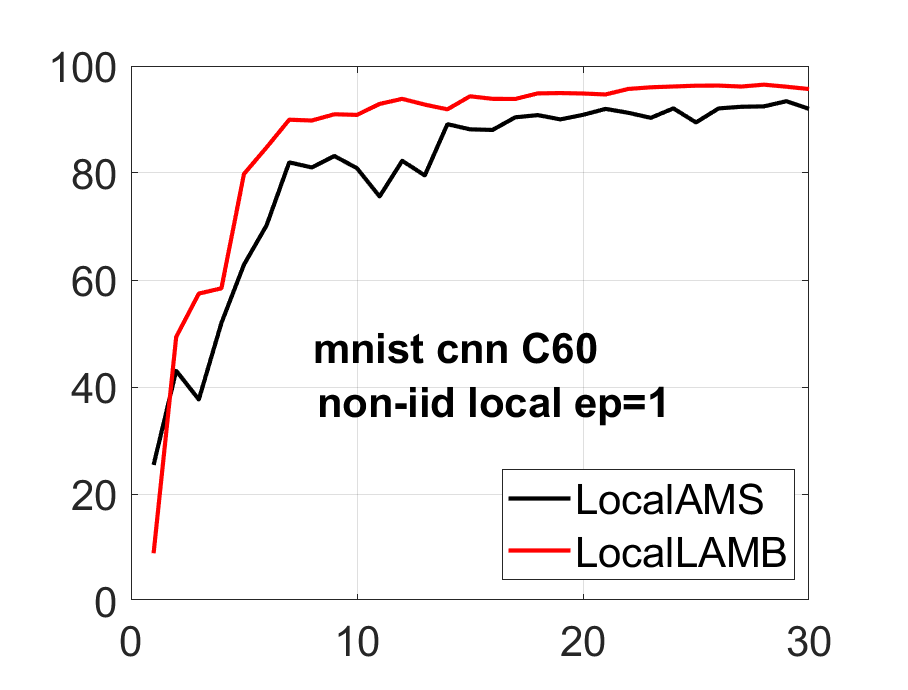
\includegraphics[width=2.5in]{figure/mnist_testerror_cnn_ep1_client60_iid0.eps}
        }
    \end{center}
    \vspace{-0.1in}
	\caption{Test accuracy on CNN + MNIST. Non-iid data distribution.}
	\label{fig:mnist-cnn-noniid}
\end{figure}

\begin{figure}[h]
    \begin{center}
        \mbox{
        \includegraphics[width=2.5in]{figure/cifar_testerror_cnn_ep1_client10_iid1.eps}
        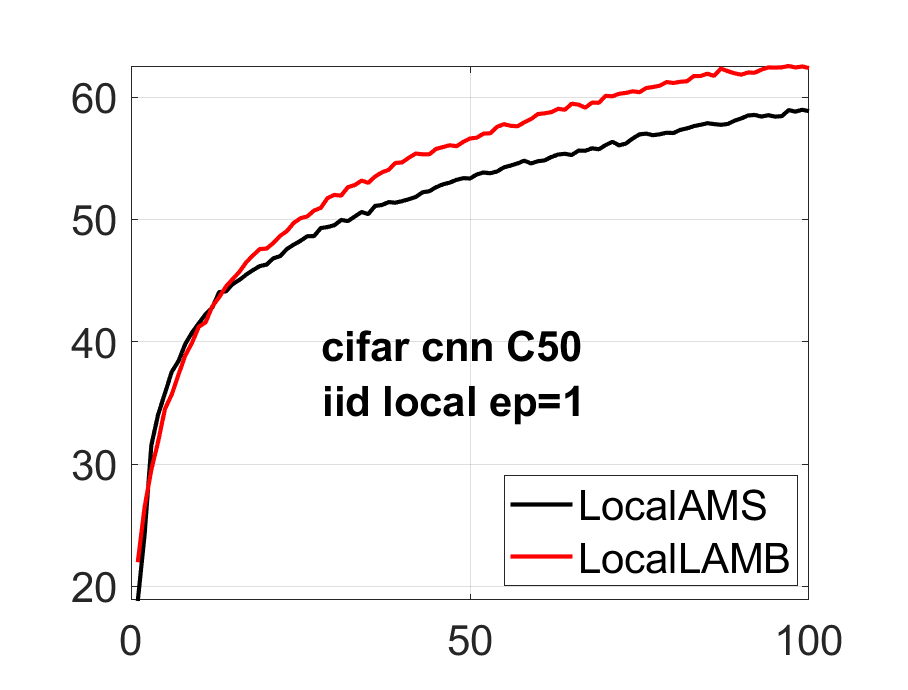
\includegraphics[width=2.5in]{figure/cifar_testerror_cnn_ep1_client50_iid1.eps}
        }
        \mbox{
        \includegraphics[width=2.5in]{figure/cifar_testerror_cnn_ep3_client10_iid1.eps}
        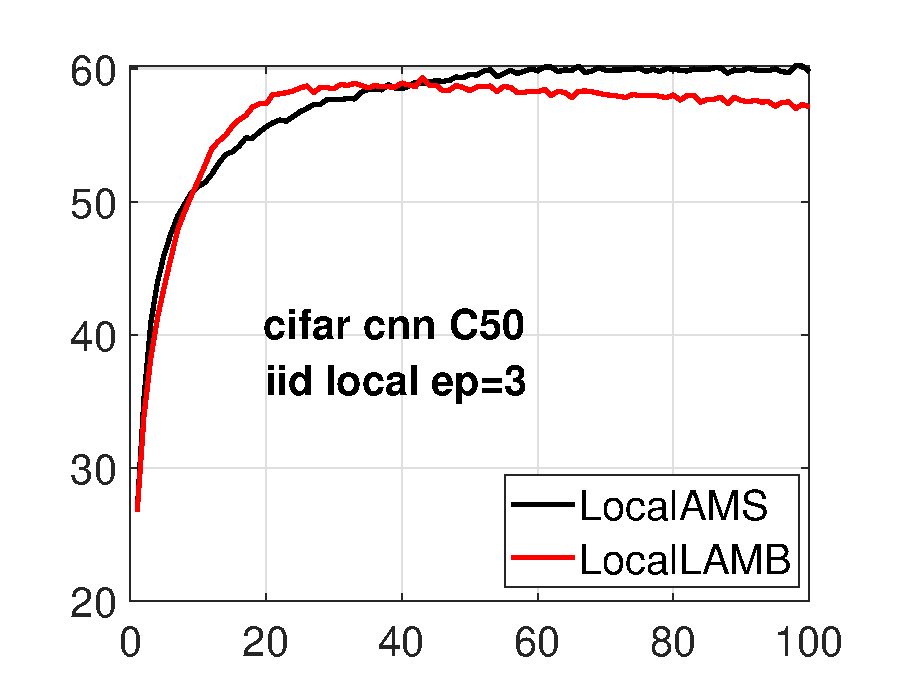
\includegraphics[width=2.5in]{figure/cifar_testerror_cnn_ep3_client50_iid1.eps}
        }
    \end{center}
    \vspace{-0.1in}
	\caption{Test accuracy on CNN + CIFAR10. iid data distribution.}
	\label{fig:cifar-cnn-iid}
\end{figure}

\begin{figure}[h]
    \begin{center}
        \mbox{
        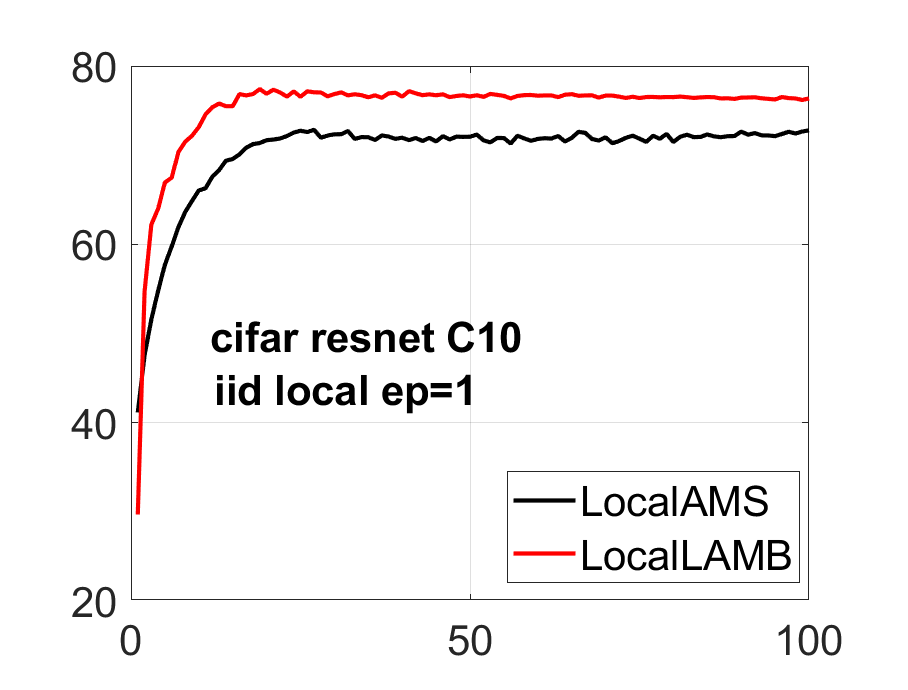
\includegraphics[width=2.5in]{figure/cifar_testerror_resnet_ep1_client10_iid1.eps}
        \includegraphics[width=2.5in]{figure/cifar_testerror_resnet_ep1_client50_iid1.eps}
        }
        \mbox{
        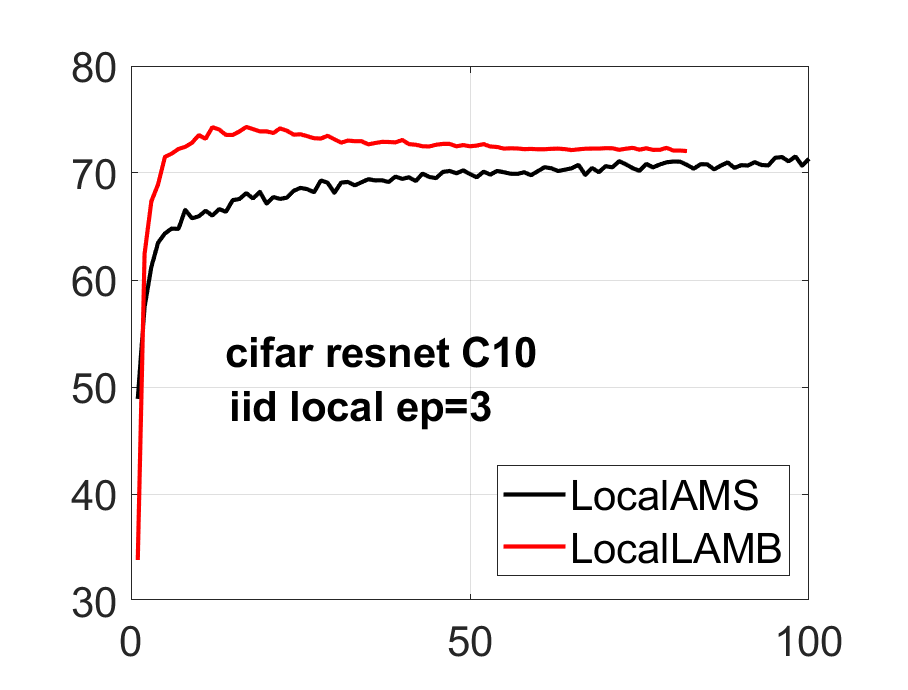
\includegraphics[width=2.5in]{figure/cifar_testerror_resnet_ep3_client10_iid1.eps}
        \includegraphics[width=2.5in]{figure/cifar_testerror_resnet_ep3_client50_iid1.eps}
        }
    \end{center}
    \vspace{-0.1in}
	\caption{Test accuracy on ResNet + CIFAR10. iid data distribution.}
	\label{fig:cifar-resnet-iid}
\end{figure}

\section{Conclusion}\label{sec:conclusion}

\newpage

\bibliographystyle{plain}
\bibliography{ref}


\appendix 

\section{Appendix}\label{sec:appendix}


%-----------------------------------------------------------------------------
%\vspace{0.4cm}

\end{document} 